\section{System Level Design}

\paragraph{}
To accomplish all the tasks necessary for this DAQ, several design choices were made at the system level.
These include decisions about what microcontroller was being used, the type of data being stored, the media device that data is being stored on, how other sensor or control nodes will communicate with the DAQ, what onboard sensors are on the DAQ, how or if the DAQ can communicate wirelessly, how a user can interface with the DAQ, and how firmware updates can be applied.

\paragraph{}
The first thing considered was how nodes can communicate with the DAQ.
The previous DAQ solution used CAN communication with a 1 Mbps data rate to collect data from all nodes on the car.
This became a throughput bottleneck, and lower priority CAN IDs would occasionally be blocked by high throughput, higher priority data.
The robustness of the CAN bus was very nice and allowed for reliable communication between all nodes on the car, so newer CAN interfaces were primarily explored.
There are currently 20 sensors and over 100 bytes of internal controls information worth of data that are desired during competition and testing that are sent from three different nodes in seven different messages.
The majority of this data is being transmitted at 400 hz.
Additionally, during testing season, there are an additional 20 sensors that are used to help validate various models and analyses.
Worst-case CAN loading for different data rates was plotted for both CAN and CAN FD in \cref{fig:CANAnalysis} to determine what data rates are acceptable.
To keep the robustness of CAN and to improve issues related to throughput, CAN FD with an arbitration rate of 1 Mbps and a data rate of 5 Mbps was selected to leave room for more future sensor or controller additions.

\begin{figure}[H]
	\centering
	\includegraphics[width=\linewidth]{CanAnalysis.png}
	\caption{CAN Bus Loading Analysis}
	\label{fig:CANAnalysis}
\end{figure}

\paragraph{}
The next consideration was how data is stored on the DAQ.
The previous DAQ solution utilized the onboard micro-SD card reader on the Teensy 3.5 \cite{TEENSY35} and Teensy 4.1 \cite{TEENSY41} microcontrollers and stored data in a CSV format.
The micro-SD card worked well with the small form factor, large number of resources available, common communication support with SPI or SDIO, and sufficient storage for 10 hours of data collection.
An alternative option would be to use an SSD.
This would allow for larger storage volumes but would add significant cost to implementation complexity, mass, physical volume, and power consumption.
As a result, a micro-SD card was selected as the storage medium.

\paragraph{}
With an SD card as the storage medium, the maximum amount of data stored is the largest constraint.
In a CSV file, each digit of a number is represented as a character, meaning that in order to represent the number "100", three bytes are required in addition to the comma delineator.
This same number can be represented with just a single byte if the data is stored in a binary format.
Knowing that the total amount of data stored during competition is nearly 200 bytes at 400 Hz, and the worst-case values for 1-byte values being three characters, 2-byte values being 5 characters, and 4-byte numbers being ten characters, the amount of data stored over a 10 hours would be 6.6 GB.
As a result, the data is stored in a binary format described in \cref{fig:MetadataDiagram}.

\begin{figure}[H]
	\centering
	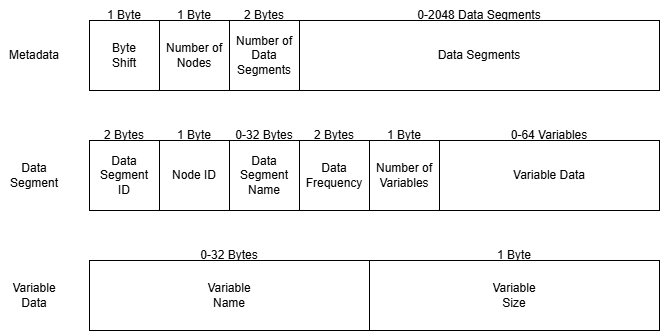
\includegraphics[width=\linewidth]{Metadata.png}
	\caption{File Metadata Byte Diagram}
	\label{fig:MetadataDiagram}
\end{figure}

\paragraph{}
To be able to parse this data, the data contained in the file is outlined at the beginning of the file, including information about data group IDs, the number of variables per ID, the size of each variable, and the name of the data associated with each variable as described in \cref{fig:MetadataDiagram}.
This header is generated dynamically at runtime, so that if new data is added to the list of logged values, DAQ firmware does not need to be modified to accommodate new data.
Each data segment is defined by the CAN message that will transmit the data.
Due to this, each data segment is a maximum of 64 bytes in size.

\paragraph{}
The selected microcontroller was the STM32H750VBT6 from ST \cite{STMProductPage}.
This microcontroller was selected for several reasons, including a vehicle-wide platform switch to STM32 microcontrollers, internal CAN FD controllers, SDIO connectivity, and a 480 MHz core frequency.
The platform switch is driven by three main criteria:
\begin{itemize}
	\item The ability to lay out the chip on a PCB
	\item Having access to the debug pins for programming and debugging
	\item Large amounts of community support and open-source libraries
\end{itemize}
Teensy development boards utilize NXP chips that have most of the same features as STM32 chips, but have slightly less community support.
Additionally, STM32 microcontrollers are used in EE 329 and CPE 316, providing experience on the platform for students who have taken those courses.

\paragraph{}
Something that all off-the-shelf data loggers do is provide the ability to connect some analog or digital sensors directly to the logger.
This functionality is desirable as it allows for a sensor to be added without external electronics, so long as the sensor output is supported by the logger.
To include similar functionality, 4 analog sensor channels are available to be directly plugged into the DAQ.
This includes a 5V source and a GND for each.
Additionally, there is an onboard IMU and GPS to be used for the common measurements of acceleration and velocity.
These sensors are on the PCB itself and require no additional wiring by a user.

\paragraph{}
The final major piece of functionality provided by the DAQ is the ability to wirelessly transmit data across a range of up to 2 miles.
This is to provide live diagnostics during testing or competition to the crew in the pits to help diagnose issues and reduce time debugging if issues occur.
To do this, a radio module was added.
To comply with FCC and competition regulations, the main options for frequency ranges were 900 MHz, 2.4 GHz, and 5 GHz.
Since competition and testing sites are often hilly and full of trees, higher frequency nodes struggle to transmit over long distances reliably.
This drove the desire to utilize a 900 MHz radio module.
The XBee 3 Pro was selected due to its wide community support and ease of integration.
\Cref{fig:SysDiagram} describes the basic way in which these components all interface together.

\begin{figure}[H]
	\centering
	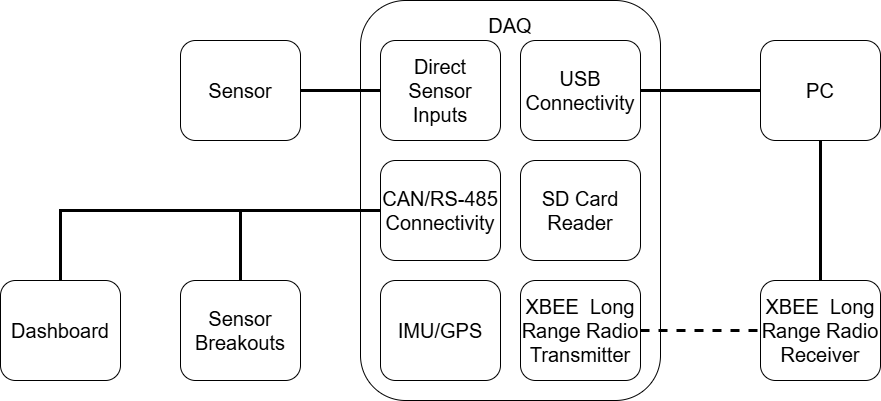
\includegraphics[width=\linewidth]{SystemDiagram.png}
	\caption{System Level Block Diagram}
	\label{fig:SysDiagram}
\end{figure}

\paragraph{}
The last major design choice was to utilize the Arduino framework for writing the firmware for the DAQ.
This was chosen to reduce the time required to write and test firmware for interfacing with the hardware.
Specifically, configuring the peripherals for CAN and SDIO is complex and would have taken development time away from higher level software features.
To use the Arduino framework, the PlatformIO \cite{PlatformIOSite} extension from VSCode \cite{VSCode} was used to setup the project.
STM32 microcontrollers utilize STM32Duino \cite{STM32DuinoGithub} as the source code for the Arduino integration.